% Ejemplo de documento LaTeX
% Tipo de documento y tamaño de letra
\documentclass[12pt]{article}


\usepackage[spanish]{babel}
\usepackage{longtable} 
\selectlanguage{spanish}
\usepackage[utf8x]{inputenc}
\usepackage{graphicx}




% EL titulo, autor y fecha del documento
\title{Reporte de Actividad 6}
\author{Carlos Medina}
\date{10-04-15}


% Aqui comienza el cuerpo del documento
\begin{document}
% Construye el título
\maketitle


El siguiente reporte describirá los pasos realizados para la actividad 7 (2015-1), se explicarán y se mostrarán los resultados de ésta.




\hspace {0.5cm} En este reporte estudiaremos las mareas, los tipos de mareas, sus comportamientos, y verémos cómo calcular las mareas altas y bajas en un periodo de tiempo como un mes e incluso un día.

\section{¿Cómo se originan?}

El origen de las fuerza de marea se debe a que la Tierra es un cuerpo extenso y el campo gravitatorio producido por la Luna o por el Sol no es homogéneo en todos sus puntos, ya que hay unos puntos que están más cercanos y otros más alejados de dichos cuerpos celestes.

 
\begin{center}
	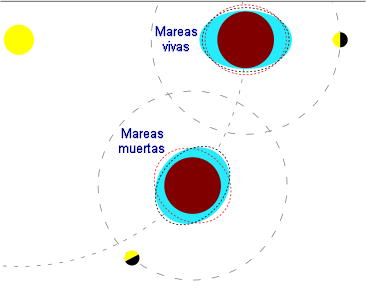
\includegraphics[width=8cm]{mar.png}\\
\end{center}
 
El elipsoide debido a las mareas solares tiene el eje mayor dirigido hacia el Sol. El elipsoide debido a las mareas lunares tiene el eje mayor dirigido hacia la Luna. Como la Luna gira alrededor de la Tierra, los ejes mayores de los elipsoides no giran a la misma velocidad.

	Con respecto a las estrellas, el periodo de rotación del elipsoide solar es de un año. El elipsoide de la Luna es de 27,32 días. El resultado es que los ejes de los dos elipsoides se acercan cada 14,7652944 días.
	
	 Cuando los ejes mayores de los dos elipsoides están alineados, la amplitud de las mareas es máxima y se llaman mareas vivas o mareas sizigias. Esto sucede en las lunas nuevas y en las lunas llenas. En cambio, cuando el eje mayor de cada elipsoide está alineado con el eje menor del otro, la amplitud de las mareas es mínima. Esto sucede en los cuartos menguantes y los cuartos crecientes. Estas mareas se llaman mareas muertas o mareas de cuadratura.
	 
	 
\section{Historia}	 
	 
	 El fenómeno de las mareas es conocido desde la antigüedad. Parece ser que Piteas (siglo IV a. C.) fue el primero en señalar la relación entre la amplitud de la marea y las fases de la Luna, así como su periodicidad. Plinio el Viejo (23-79) en su Naturalis Historia describe correctamente el fenómeno y piensa que la marea está relacionada con la Luna y el Sol. 

 
\begin{center}
	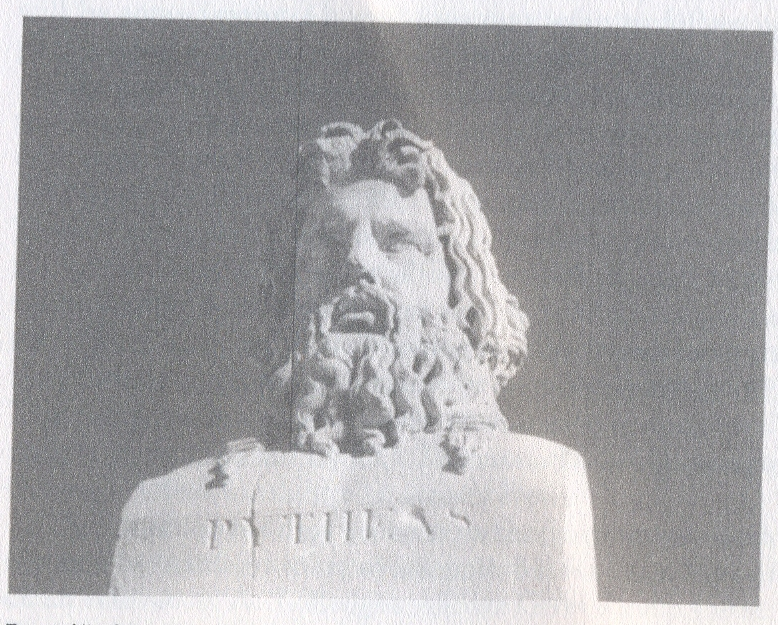
\includegraphics[width=5cm]{piteas.png}\\
\end{center}	 
	 
	 Mucho más tarde, Bacon, Kepler y otros trataron de explicar ese fenómeno, admitiendo la atracción de la Luna y del Sol. Pero fue Isaac Newton en su obra Philosophiae Naturalis Principia Mathematica («Principios matemáticos de la Filosofía Natural», 1687) quien dio la explicación de las mareas aceptada actualmente. Más tarde, Pierre-Simon Laplace (1749-1827) y otros científicos ampliaron el estudio de las mareas desde un punto de vista dinámico.

Isaac Newton realizó varios estudios científicos del comportamiento de las mareas y calculó la altura de éstas según la fecha del mes, la estación del año y la latitud. Más tarde, Simon Laplace complementó los estudios de Newton.
	 
	 \begin{center}
	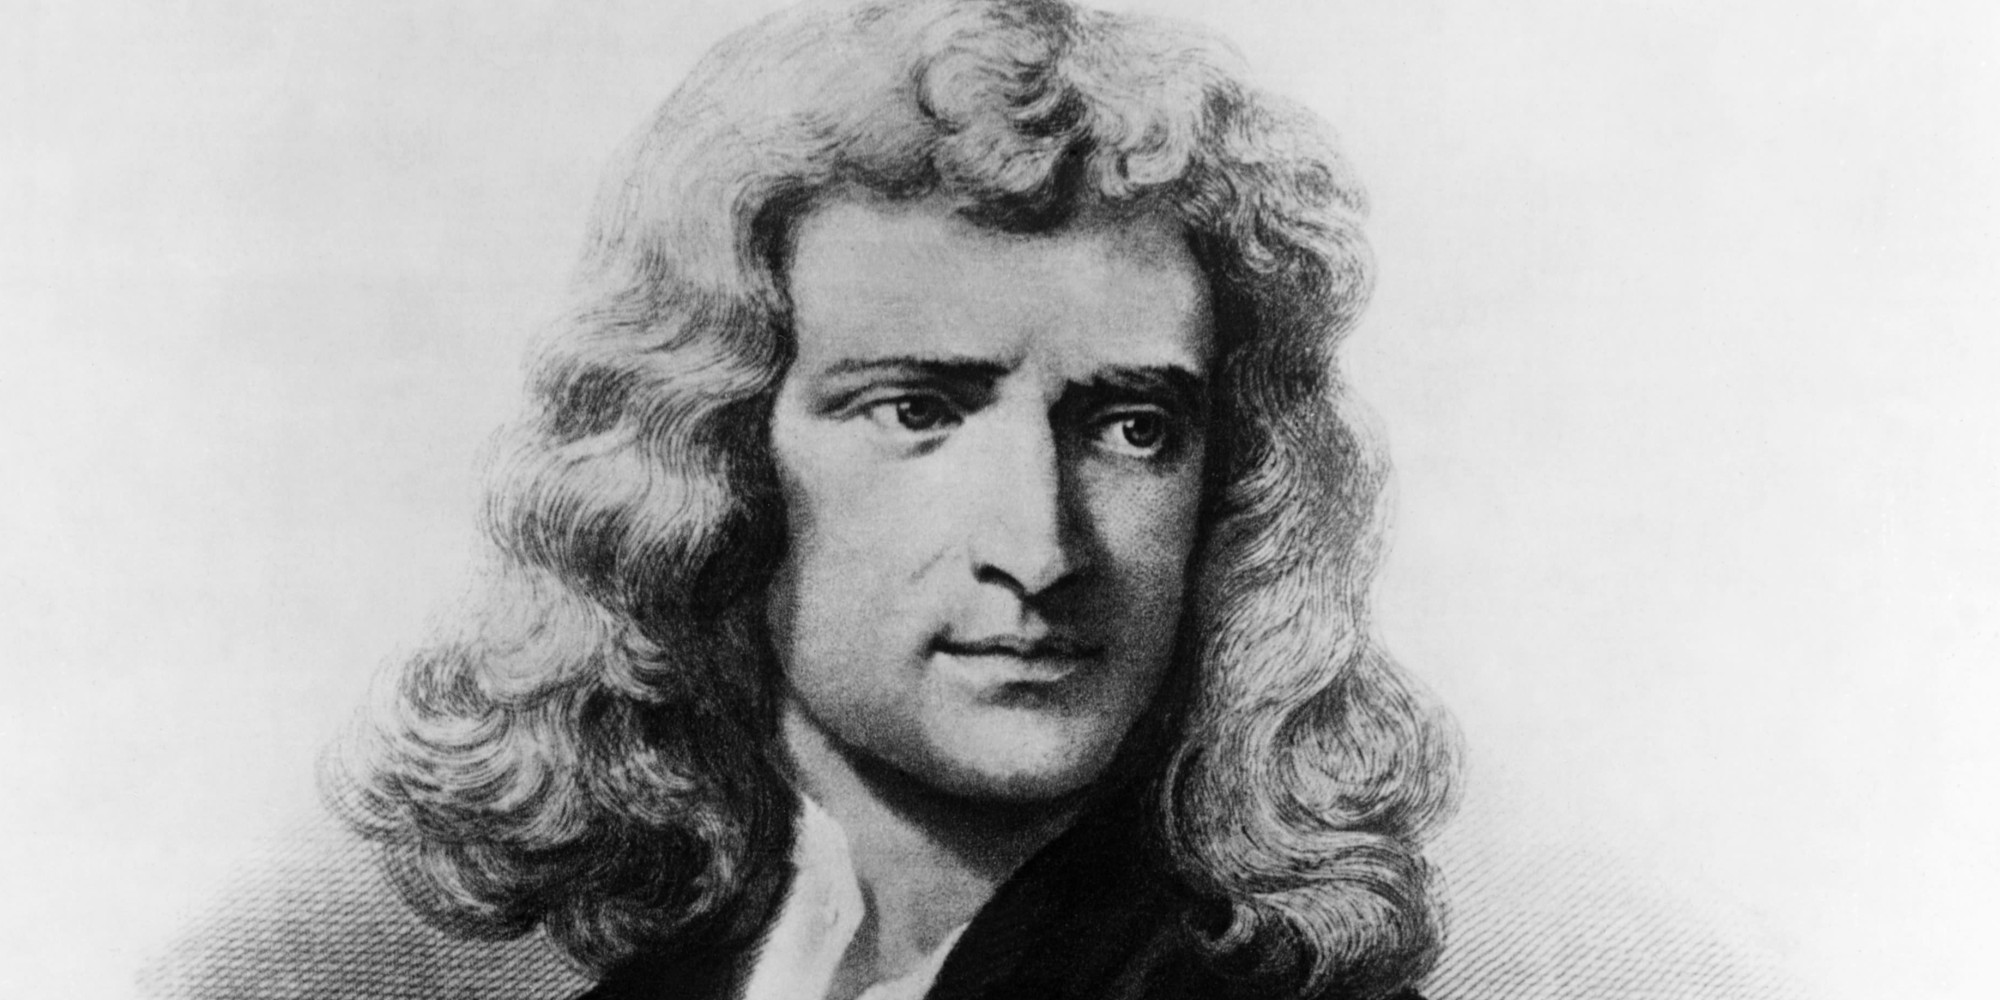
\includegraphics[width=8cm]{niuton.jpg}\\
\end{center}	 
	 
\section{Analizando las mareas}

	Ahora, analizaremos un ejemplo de mareas reales con un archivo con datos que nos ha proporcionado el Dr. Julio César Rodríguez, del Departamento de Agricultura. Los datos se proporcionan en un archivo en formato de Excel, que puedes descargar de aquí. Los datos corresponden al manglar El Sargento, ubicado en la costa, cerca del Desemboque de los Seris, casi frente a la Isla del Tiburón.
	
		 \begin{center}
	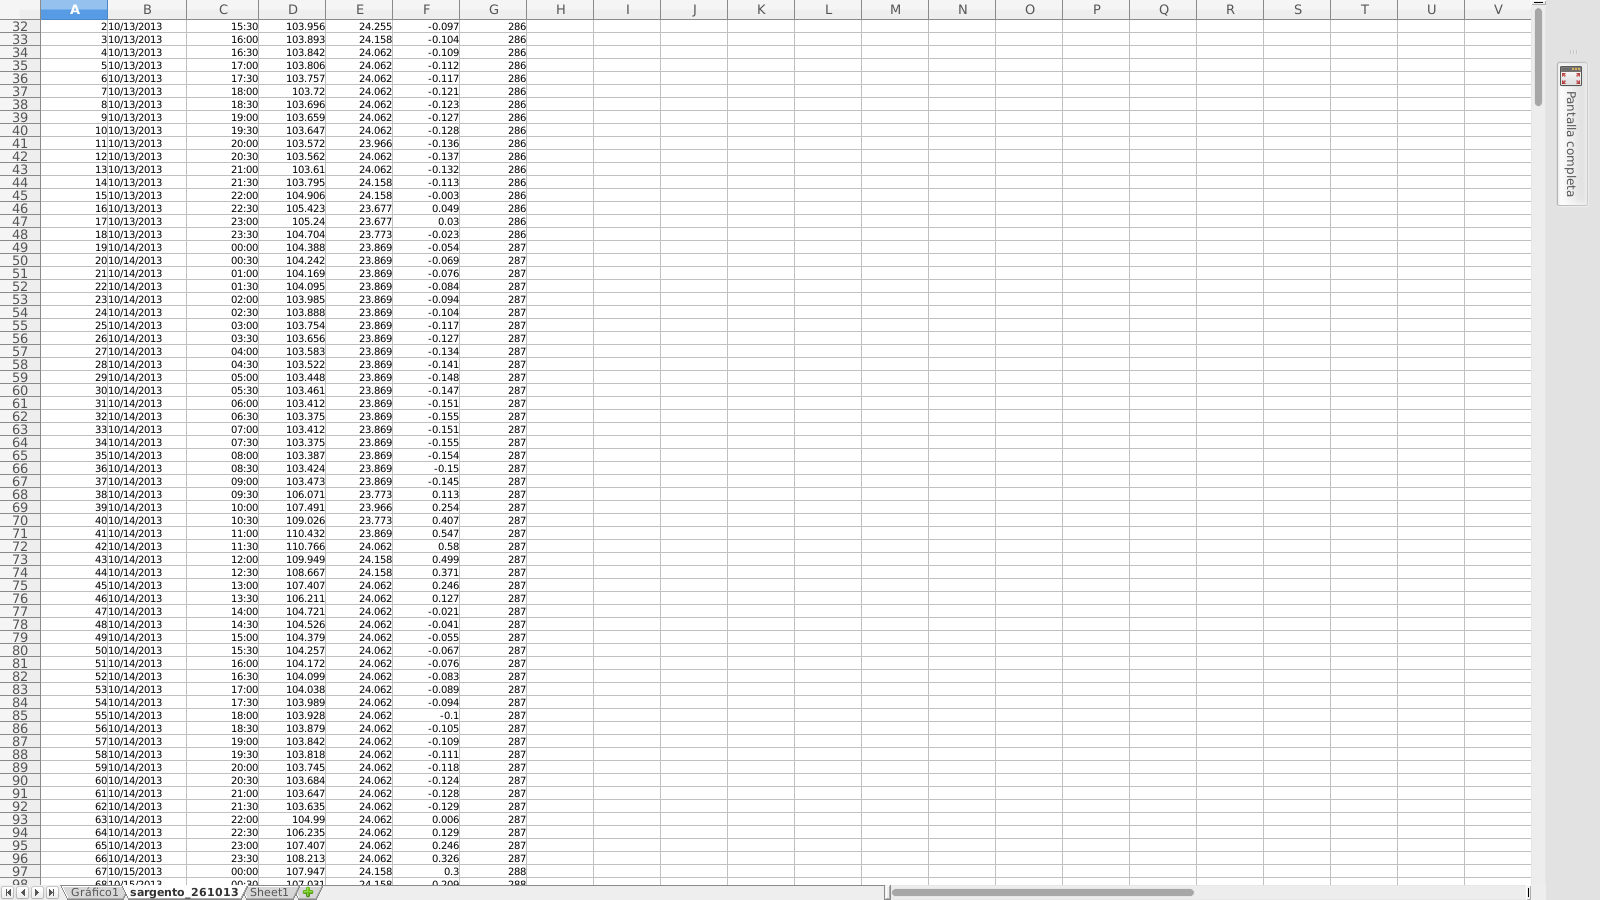
\includegraphics[width=20cm]{d.png}\\
\end{center}	 
	
	Primeramente, procedemos a procesar los datos de una forma que fortran los pueda leer.
	
		 \begin{center}
	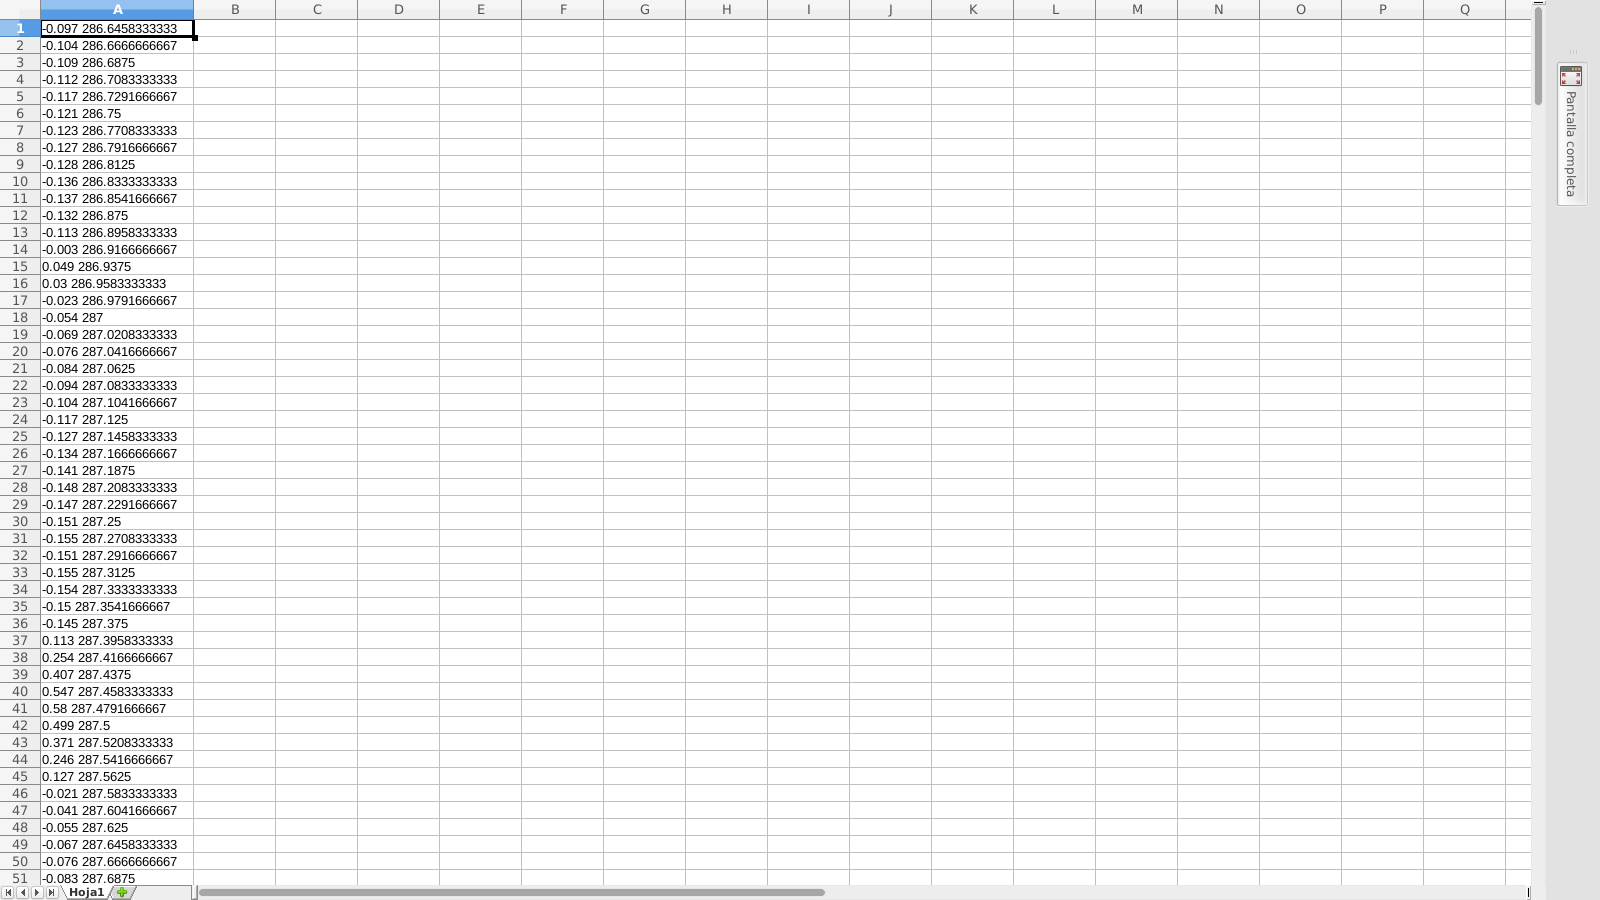
\includegraphics[width=20cm]{d2.png}\\
\end{center}	 

Ahora, proseguimos con

\end{document}
